 
% *************** LEd - MSc template document ***************

\documentclass[11pt, oneside, a4paper, oldfontcommands]{memoir}
% *************** Document style definitions ***************

% ******************************************************************
% This file defines the document design.
% Usually it is not necessary to edit this file, but you can change
% the design if you want.
% ******************************************************************

% *************** Load packages ***************
\usepackage{graphicx}
\usepackage{epsfig}
\usepackage{amsmath}
\usepackage{amssymb}
\usepackage{amsthm}
\usepackage{booktabs}
\usepackage{stmaryrd}
\usepackage{url}
\usepackage{longtable}
\usepackage[figuresright]{rotating}
\usepackage{textcomp}
\usepackage{listings}
\usepackage[utf8x]{inputenc}

\usepackage{natbib}
\bibpunct{[}{]}{;}{s}{,}{,}
\usepackage[colorlinks=true, linkcolor=blue, citecolor=blue]{hyperref}

% *************** Enable index generation ***************
\makeindex

% *************** Add reference to page number at which bibliography entry is cited ***************
\usepackage{citeref}
\renewcommand{\bibitempages}[1]{\newblock {\scriptsize [\mbox{cited at p.\ }#1]}}

% *************** Some colour definitions ***************
\usepackage{color}

\definecolor{greenyellow}   {cmyk}{0.15, 0   , 0.69, 0   }
\definecolor{yellow}        {cmyk}{0   , 0   , 1   , 0   }
\definecolor{goldenrod}     {cmyk}{0   , 0.10, 0.84, 0   }
\definecolor{dandelion}     {cmyk}{0   , 0.29, 0.84, 0   }
\definecolor{apricot}       {cmyk}{0   , 0.32, 0.52, 0   }
\definecolor{peach}         {cmyk}{0   , 0.50, 0.70, 0   }
\definecolor{melon}         {cmyk}{0   , 0.46, 0.50, 0   }
\definecolor{yelloworange}  {cmyk}{0   , 0.42, 1   , 0   }
\definecolor{orange}        {cmyk}{0   , 0.61, 0.87, 0   }
\definecolor{burntorange}   {cmyk}{0   , 0.51, 1   , 0   }
\definecolor{bittersweet}   {cmyk}{0   , 0.75, 1   , 0.24}
\definecolor{redorange}     {cmyk}{0   , 0.77, 0.87, 0   }
\definecolor{mahogany}      {cmyk}{0   , 0.85, 0.87, 0.35}
\definecolor{maroon}        {cmyk}{0   , 0.87, 0.68, 0.32}
\definecolor{brickred}      {cmyk}{0   , 0.89, 0.94, 0.28}
\definecolor{red}           {cmyk}{0   , 1   , 1   , 0   }
\definecolor{orangered}     {cmyk}{0   , 1   , 0.50, 0   }
\definecolor{rubinered}     {cmyk}{0   , 1   , 0.13, 0   }
\definecolor{wildstrawberry}{cmyk}{0   , 0.96, 0.39, 0   }
\definecolor{salmon}        {cmyk}{0   , 0.53, 0.38, 0   }
\definecolor{carnationpink} {cmyk}{0   , 0.63, 0   , 0   }
\definecolor{magenta}       {cmyk}{0   , 1   , 0   , 0   }
\definecolor{violetred}     {cmyk}{0   , 0.81, 0   , 0   }
\definecolor{rhodamine}     {cmyk}{0   , 0.82, 0   , 0   }
\definecolor{mulberry}      {cmyk}{0.34, 0.90, 0   , 0.02}
\definecolor{redviolet}     {cmyk}{0.07, 0.90, 0   , 0.34}
\definecolor{fuchsia}       {cmyk}{0.47, 0.91, 0   , 0.08}
\definecolor{lavender}      {cmyk}{0   , 0.48, 0   , 0   }
\definecolor{thistle}       {cmyk}{0.12, 0.59, 0   , 0   }
\definecolor{orchid}        {cmyk}{0.32, 0.64, 0   , 0   }
\definecolor{darkorchid}    {cmyk}{0.40, 0.80, 0.20, 0   }
\definecolor{purple}        {cmyk}{0.45, 0.86, 0   , 0   }
\definecolor{plum}          {cmyk}{0.50, 1   , 0   , 0   }
\definecolor{violet}        {cmyk}{0.79, 0.88, 0   , 0   }
\definecolor{royalpurple}   {cmyk}{0.75, 0.90, 0   , 0   }
\definecolor{blueviolet}    {cmyk}{0.86, 0.91, 0   , 0.04}
\definecolor{periwinkle}    {cmyk}{0.57, 0.55, 0   , 0   }
\definecolor{cadetblue}     {cmyk}{0.62, 0.57, 0.23, 0   }
\definecolor{cornflowerblue}{cmyk}{0.65, 0.13, 0   , 0   }
\definecolor{midnightblue}  {cmyk}{0.98, 0.13, 0   , 0.43}
\definecolor{navyblue}      {cmyk}{0.94, 0.54, 0   , 0   }
\definecolor{royalblue}     {cmyk}{1   , 0.50, 0   , 0   }
\definecolor{blue}          {cmyk}{1   , 1   , 0   , 0   }
\definecolor{cerulean}      {cmyk}{0.94, 0.11, 0   , 0   }
\definecolor{cyan}          {cmyk}{1   , 0   , 0   , 0   }
\definecolor{processblue}   {cmyk}{0.96, 0   , 0   , 0   }
\definecolor{skyblue}       {cmyk}{0.62, 0   , 0.12, 0   }
\definecolor{turquoise}     {cmyk}{0.85, 0   , 0.20, 0   }
\definecolor{tealblue}      {cmyk}{0.86, 0   , 0.34, 0.02}
\definecolor{aquamarine}    {cmyk}{0.82, 0   , 0.30, 0   }
\definecolor{bluegreen}     {cmyk}{0.85, 0   , 0.33, 0   }
\definecolor{emerald}       {cmyk}{1   , 0   , 0.50, 0   }
\definecolor{junglegreen}   {cmyk}{0.99, 0   , 0.52, 0   }
\definecolor{seagreen}      {cmyk}{0.69, 0   , 0.50, 0   }
\definecolor{green}         {cmyk}{1   , 0   , 1   , 0   }
\definecolor{forestgreen}   {cmyk}{0.91, 0   , 0.88, 0.12}
\definecolor{pinegreen}     {cmyk}{0.92, 0   , 0.59, 0.25}
\definecolor{limegreen}     {cmyk}{0.50, 0   , 1   , 0   }
\definecolor{yellowgreen}   {cmyk}{0.44, 0   , 0.74, 0   }
\definecolor{springgreen}   {cmyk}{0.26, 0   , 0.76, 0   }
\definecolor{olivegreen}    {cmyk}{0.64, 0   , 0.95, 0.40}
\definecolor{rawsienna}     {cmyk}{0   , 0.72, 1   , 0.45}
\definecolor{sepia}         {cmyk}{0   , 0.83, 1   , 0.70}
\definecolor{brown}         {cmyk}{0   , 0.81, 1   , 0.60}
\definecolor{tan}           {cmyk}{0.14, 0.42, 0.56, 0   }
\definecolor{gray}          {cmyk}{0   , 0   , 0   , 0.50}
\definecolor{black}         {cmyk}{0   , 0   , 0   , 1   }
\definecolor{white}         {cmyk}{0   , 0   , 0   , 0   } 

% *************** Enable hyperlinks in PDF documents ***************
%\ifpdf
%    \pdfcompresslevel=9
%        \usepackage[plainpages=false,pdfpagelabels,bookmarksnumbered,%
%        colorlinks=true,%
%        linkcolor=sepia,%
%        citecolor=sepia,%
%        filecolor=maroon,%
%        pagecolor=red,%
%        urlcolor=sepia,%
%        pdftex,%
%        unicode]{hyperref} 
%    \input supp-mis.tex
%    \input supp-pdf.tex
%    \pdfimageresolution=600
%    \usepackage{thumbpdf} 
%\else
%    \usepackage{hyperref}
%\fi

\usepackage{memhfixc}

% *************** Page layout ***************
\settypeblocksize{*}{32pc}{1.618}

\setlrmargins{*}{1.47in}{*}
\setulmargins{*}{*}{1.3}

\setheadfoot{\onelineskip}{2\onelineskip}
\setheaderspaces{*}{2\onelineskip}{*}

\def\baselinestretch{1.1}

\checkandfixthelayout

% *************** Chapter and section style ***************
\makechapterstyle{mychapterstyle}{%
    \renewcommand{\chapnamefont}{\LARGE\sffamily\bfseries}%
    \renewcommand{\chapnumfont}{\LARGE\sffamily\bfseries}%
    \renewcommand{\chaptitlefont}{\Huge\sffamily\bfseries}%
    \renewcommand{\printchaptertitle}[1]{%
        \chaptitlefont\hrule height 0.5pt \vspace{1em}%
        {##1}\vspace{1em}\hrule height 0.5pt%
        }%
    \renewcommand{\printchapternum}{%
        \chapnumfont\thechapter%
        }%
}

\chapterstyle{mychapterstyle}

\setsecheadstyle{\Large\sffamily\bfseries}
\setsubsecheadstyle{\large\sffamily\bfseries}
\setsubsubsecheadstyle{\normalfont\sffamily\bfseries}
\setparaheadstyle{\normalfont\sffamily}

\makeevenhead{headings}{\thepage}{}{\small\slshape\leftmark}
\makeoddhead{headings}{\small\slshape\rightmark}{}{\thepage}

% *************** Table of contents style ***************
\settocdepth{subsection}

\setsecnumdepth{subsection}
\maxsecnumdepth{subsection}
\settocdepth{subsection}
\maxtocdepth{subsection}

% ********** Commands for epigraphs **********
\setlength{\epigraphwidth}{0.57\textwidth}
\setlength{\epigraphrule}{0pt}
\setlength{\beforeepigraphskip}{1\baselineskip}
\setlength{\afterepigraphskip}{2\baselineskip}

\newcommand{\epitext}{\sffamily\itshape}
\newcommand{\epiauthor}{\sffamily\scshape ---~}
\newcommand{\epititle}{\sffamily\itshape}
\newcommand{\epidate}{\sffamily\scshape}
\newcommand{\episkip}{\medskip}

\newcommand{\myepigraph}[4]{%
	\epigraph{\epitext #1\episkip}{\epiauthor #2\\\epititle #3 \epidate(#4)}\noindent}

% *************** Other ***************
\renewcommand{\thefootnote}{\fnsymbol{footnote}}

\lstset
{
language=C++,
frame=tb,
framesep=5pt,
basicstyle=\normalsize,
keywordstyle=\ttfamily\color{navyblue},
identifierstyle=\ttfamily\color{black}\bfseries, 
commentstyle=\color{brown},
stringstyle=\ttfamily,
showstringspaces=false,
tabsize=4,
numbers=left,
stepnumber=1,
numberstyle=\small,
numbersep=10pt,
}

% *************** End of document style definition ***************


\usepackage{wrapfig}
\usepackage{listings}
\usepackage{pifont}
\newcommand{\tick}{\ding{52}} 
\begin{document}
% *************** Front matter ***************
\frontmatter
% *************** Front matter ***************

% ***************************************************
% You should specify the contents of title page here
% Then you can specify dedication page or disable it
% ***************************************************

% *************** Title page ***************
\pagestyle{empty}
\sffamily

\noindent
\begin{center}
    \Large
    University Politehnica of Bucharest\\
    Faculty of Automatic Control and Computers \\
    Computer Science and Engineering Department \\
\end{center}

%\vfill\vfill 
		\par\vspace*{3mm}
		\begin{table*}[h]
        	\begin{center}
				\begin{tabular}{cccc}
                    
\includegraphics[width=0.13\textwidth]{frontbackstyle/upb}
					& & &
					
\includegraphics[width=0.30\textwidth]{frontbackstyle/cs}
            	\end{tabular}
			\end{center}
		\end{table*}
		
		\par\vspace*{15mm}

\begin{center}
    \Large
    BACHELOR THESIS\\
\end{center}

\vfill
\begin{center}
	\HUGE\bfseries
	Mobile Gateway for Wireless Sensor Networks utilizing drones\\
\vfill
	\large
	
\end{center}

\vfill
\begin{center}
    \Large
    by
\end{center}

\vfill
\begin{center}
    \huge\bfseries
    Ioan Deaconu
\end{center}

\vfill\vfill\vfill
\begin{center}
	\Large
	Supervisor: As. Drd. Ing. Andrei Voinescu
	%Supervisor: S.l. Dr. Ing. Emil Slu\c{s}anschi\\
\end{center}

\vfill
\par\vspace*{15mm}
\begin{center}
\large
    Bucharest, September 2014
\end{center}

\cleardoublepage

% *************** Table of contents ***************
\pagenumbering{roman}
\pagestyle{headings}
\tableofcontents

% *************** End of front matter ***************







% *************** Main matter ***************
\mainmatter
%\nocite{*}
Wireless sensor networks are a cheap and versatile solution for monitoring various environments 
and elements of an environment. There exists a number of such applications used worldwide to monitor 
areas in which human access is hard or near impossible. The issue with these applications is that 
they are mainly used by government organizations or for research purposes. They seldom focus on 
using the data in the interest of safety for the population, such as warning them of natural 
disasters or assessing the risk of damaged areas left in the wake of a natural disaster. The 
solution we propose in this article is a low power, low cost wireless sensor which is used to 
monitor earthquakes and the status of urban structures exposed to earthquakes or other sources 
of vibration in order to prevent possible disasters.

\chapter{Introduction}
\chapter{Related Work}
\chapter{Hardware Platform}
Voi folosi o super-referință S-MAC\cite{hui} și un rahat \cite{rahat2001candidate}
\chapter{Software Platform}
\begin{figure}[ht]
 \begin{center}
  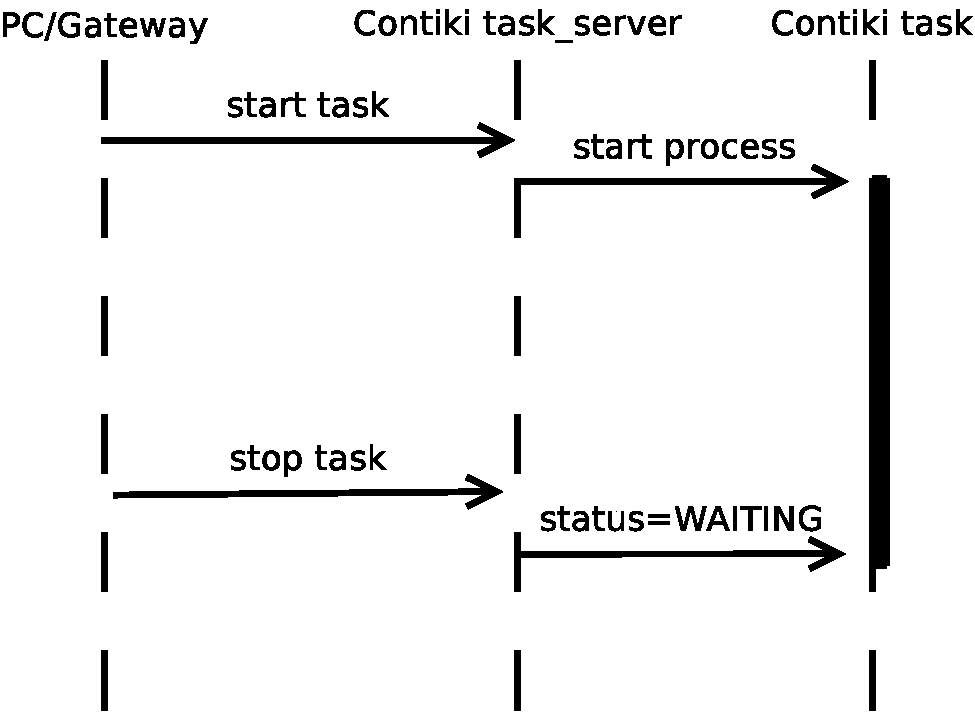
\includegraphics[scale=0.5]{img/starttask.pdf}
 \end{center}
 \caption{\small \itshape{The exchange of messages while starting/stopping tasks}}
\end{figure}


\lstset{numbers=left, mathescape=true, nolol=false,caption=Task server snippet,label=lst:taskserver}
\begin{lstlisting}
PROCESS_THREAD(task_server_process, ev, data)
{
	PROCESS_BEGIN();

	list_init(task_list);

	list_add(task_list,&el_monitor_process);
	list_add(task_list,&el_delay_process);
	list_add(task_list,&el_temperature_sensing);

	tcp_listen(HTONS(1010));

	while(1) 
	{
		PROCESS_WAIT_EVENT_UNTIL(ev == tcpip_event);

		if(uip_connected()) 
		{
			PSOCK_INIT(&ps, buffer, sizeof(buffer));

			while(!(uip_aborted() || uip_closed() 
			    || uip_timedout())) 
			{
				PROCESS_WAIT_EVENT_UNTIL
				      (ev == tcpip_event);
				handle_connection(&ps);
			}
		}
	}
	PROCESS_END();
}
\end{lstlisting}

\chapter{Other Chapters, TBD}
\chapter{Conclusions and Future Work}
% all chapters should be in a different text file
%\normalfont\normalsize
\chapter{Related Work}

The related work is starting the expand and new researches propose new ideas, but generaly speaking they tend to focus on ways of collecting the data from the nodes. The objective in their articles is to see if an UAV can be integreated with a wireless sensor networks. The conclusion is generaly positive, but a big problem in adopting their research in real life scenarios is represented by the high costs of the equipment they used and the necesary knowledge required to setup and operate the equipment.

The general experiments presented in the UAV and WSN integeration research are the following:

\begin{itemize}

\item Usign nodes signal to perform course corections for dynamic navigation
\item Data muling from nodes 
\item Using drones to deploy a new node in order to expand or to fix a problem in the network
\item Using drones to determine ground military activity \cite{akyildiz2002wireless}

\end{itemize}


\section{Standard WSN Protocols}

The protocols implemented in Wireless Sensor Network are based on sourounding node discovery in order to build a topology and find the best way they can multihop data to the gateway. This approach works best in a static environment, but in a dynamic environment or an eviroment were the distance between nodes is too big or the time between two data packets is too big, the network convergence will be slow or not even possible.

\section{UAV experiments with Wireless Sensor Networks} \cite{teh2008experiments} 

The experiment consisted of using ground nodes that had a gps position assigned. The UAV plane would performe course corection after receiving the curent gps position from the node in order to calculate the best path for muling the data from the nodes.

The advantage of using a plane used for the experiment is the longer range and higher speed that it can offer against a quadcopter or a similiar design.  But the high speed creates the problem of maneuverability. The plane has a turning range of 400 meters while the drone can almost turn on the same spot.

\section{Crop Monitoring} \cite{valente2011air}

A research of using a drone for crop monitoring has been conducted at a vineyard. Their system was comprised of a unmanned quadcopter, an Arduino board with a GPRS module for long distance communication with  the drone and ZigBee and Crossbow’s TelosB as wireless sensing nodes. The drone was not controlled via the long-distance link, but through a Spektrum DX7SE 2.4 GHz remote control.

They demonstrated that a preprogramed UAV can be used to monitor multiple crops where a standard WSN could not be deployed because of the unique constrains imposed by the environment.

The cost of the implementation was relatively high compared to ours, the remote is 300\$, the same as the entire drone that we propose and the TelosB is 99\$. This data suggests that for their experiment the drone, communication module and the remote control were half the cost of the equipment.

Another problem was that they were not saving the data localy, but sending it back to the base station where it was proccesed and saved. This can represent a problem because the system cannot function propely unless a base station is supplied.

\section{Aware platform}\cite{ollero2007aware}

The Aware platform, proposed by Ays. Egül Tüysüz Erman, Lodewijk Van Hoesel and Paul Havinga from University of Twente, is a platform that integrates WSNs, UAVs, and actuators into a disaster response setting and provides facilities for event detection, autonomous network repair by UAVs, and quick response by integrated operational forces.

They use multiple UAVs to deploy new nodes that will replace the damaged ones and check if they function. The entire system still relies on a sink to collect the data and to send them to a base station.\cite{erman2008enabling}

%\label{chap:impl}

\subsection{Placing Algorithm}
 
The placing algorithm is at its core a genetic algorithm \cite{back1997handbook} which uses
a specified set of heuristic functions to compute the fitness of individuals.
An individual is represented by the configuration of the graph at a certain, i.e.
the location of each node.

The idea behind the algorithm is to try and place the graph in a natural way, similar
to how a human would do it by hand. Because every person prefers a different type of 
layout or arrangement, the placing algorithm uses constraints specified by the user
to verify if the graph has been properly placed.

The algorithm starts by creating a generation composed of individuals which have 
been randomly placed on the canvas. It then proceeds to check how good each 
individual is by computing its fitness. This will yield a subset of layouts which
are the closest aproximation of what the user desired. At this point, for each 
part of individual (i.e. a node) it further computes a score, depending on the
number of connections and where it has been placed. Then, two individuals are 
picked and a recombination will be performed. Four new individuals shall be obtained:
one which has the best positions from both parents, one which has the worst positions
from each parent and the last two which have the best from one parent and the 
worst from the other, and vice-versa.

At the end of recombination, a new generation will have been obtained. This selective 
evolution process \cite{back1996evolutionary} will continue until either stability has been achieved (there is an
individual with the best fitness which appears constantly in every generation) or, for 
performance reasons, a certain number of generations has passed. The individual with 
the best fitness shall represent the final layout.

\subsection{Routing Algorithm}

The routing algorithm is based on the orthogonal edge routing. This method ensures 
that all the edges which compose a connection path are orthogonal. Also, another 
imposed restriction is that, when possible, no path should cross another path to 
avoid creating confusing intersection points.

The algorithm mixes a shortest path approach with an original take on avoiding obstacles.
At first, in order to route a path, the shortest path between the two components that have 
to be connected is computed, ensuring that it avoids obstacles. Then, all redundant points 
are eliminated (a redundant point is any point C which is on a valid segment [AB]). After 
this step, the path is "orthogonalized", meaning that all edges which are not orthogonal are 
broken into smaller, orthogonal edges. Should any of these new segments intersect an obstacle,
that segment shall be treated as a separate route and re-computed so that it no longer 
intersects the obstacle.

Should the computed path intersect any other already existing path, a new one shall be 
computed. It will no longer be the shortest, but it will trade area covered by the drawing 
for clarity and better understanding of the graph.

\begin{figure}[ht] \centering
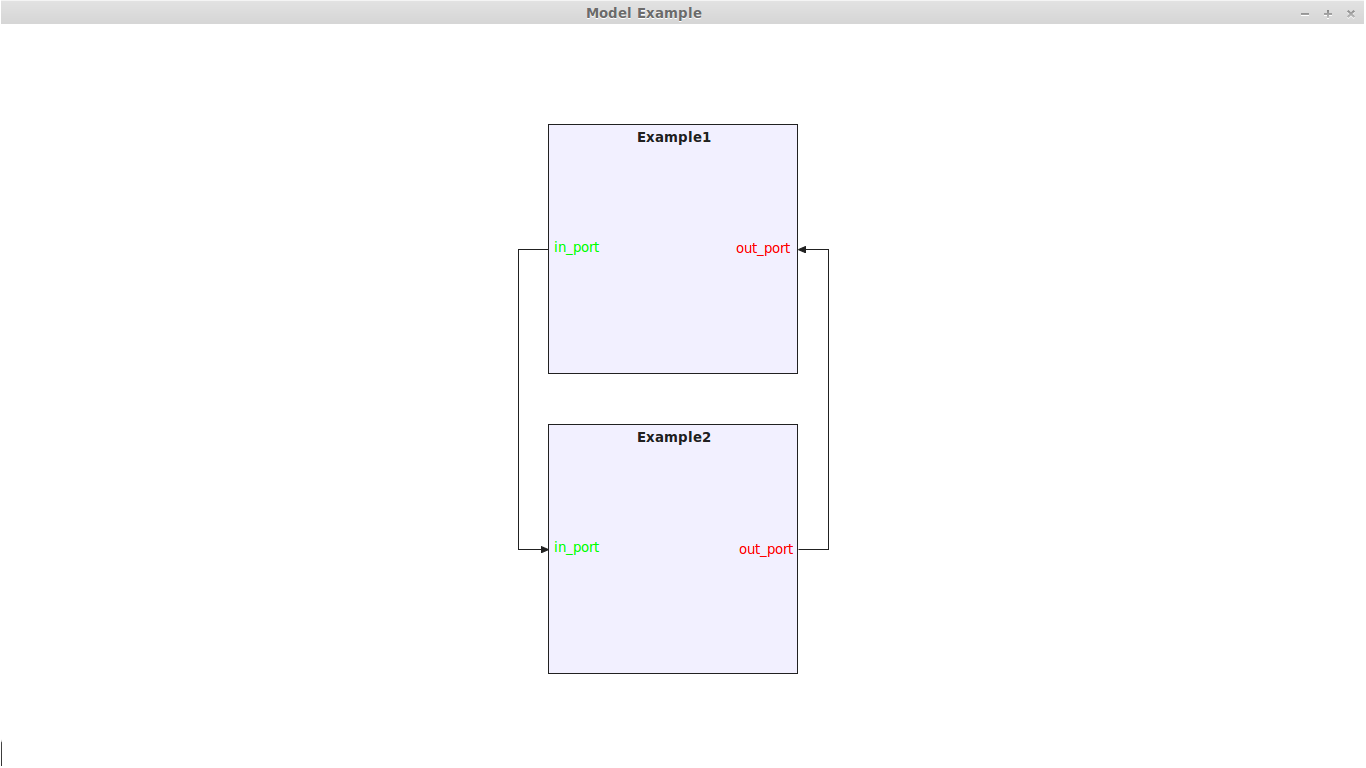
\includegraphics[width=0.5\textwidth]{src/modelExample.png}
\caption{The general look of nodes and routes in the model. Input ports are highlited green; output ports are highlighted red; arrow decorations are placed 
at the end of a route to show its direction.} \end{figure}

%\label{chap:results}

In this chapter we will cover the results obtained with this gateway platform
and other possible applications.

\begin{figure}[ht] \centering
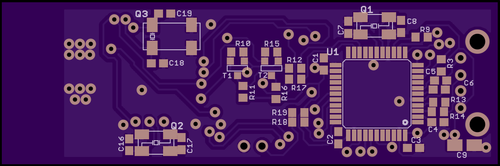
\includegraphics[width=0.3\textwidth]{img/dongleb.png} \caption{Bottom side of
SparrowDongle PCB} \end{figure}


\begin{figure}[ht] \centering
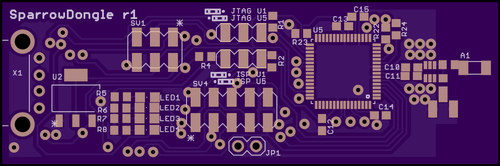
\includegraphics[width=0.3\textwidth]{img/donglef.png} \caption{Top side of
SparrowDongle PCB} \end{figure}

\subsection{Performance}

Throughput testing was done with back-to-back packets sent at 250kbps over
2.4GHz with one sending node in acceptable range, with no losses. This is due
to the double-buffering used in receiving packets from the wireless network.
As soon as one packet ends, a signal is sent to the radio controller unit with
a small delay of 9$\mu S$. Even if a new packet starts in that small interval,
receipt of the new packet goes unhindered as the first bytes of the old packet
have already been transfered to a different memory location from which they
will be sent to the USB controller unit via the serial connection.

\subsection{Software configurations}

A great advantage of using a dedicated USB Controller Unit for the gateway is
that it can be programmed as one of several USB Communication Classes. The USB
Controller Unit is not limited in implementing any of these classes since most
of the computing power at its disposal is reserved for USB.  SparrowDongle can
appear as different USB devices:

\begin{itemize}

\item \textit{Virtual Serial Port}: Communication with the wireless island
around the gateway can be made via a serial link, incoming packets will appear
on the receive end of this port and packets will be sent on the transmit end.
In typical Unix fashion, our implementation sends packet in ASCII for ease of
use and debugging. They are converted to binary form on the Radio Controller
Unit of the gateway

\item \textit{Ethernet Emulation}: In this fashion, packets are received on the
gateway and then encapsulated in an Ethernet packet sent over the USB link
(Ethernet is emulated between the USB device and USB host)

\item \textit{Network card}: SparrowDongle behaves as a wireless network card,
the operating system will register a network interface for the gateway and
addresses assigned to this interface will change the gateway's address in the
wireless medium (as opposed to changing the address for the emulated Ethernet)

\item \textit{Mass Storage}: SparrowDongle can offer a virtual filesystem
interface for innovative data acquisition from the wireless sensor network. In
accordance with the Unix philosophy of "everything is a file", the virtual
filesystem offered by the USB stick could have a file for each wireless node
where it stores recent data (as much as the gateway can store in its volatile
memory, 1-2 records per node). The software implementation for this interface
is under development.

 \end{itemize}

\subsection{Applications}


The versatility of the SparrowDongle gateway platform allows it to be deployed
in a wide range of applications, whether the gateway has to be connected to a
PC or a small embedded device, whether it has to implement a virtual serial
connection or to emulate an ethernet link.

For instance, these are the application in which SparrowDongle is currently
deployed:

 \begin{itemize} 

\item Collecting data from the sensors \cite{fcint}

\item Debuging a wireless sensor network by checking which node is working, the connection logs and the physical state of the device

\item Search and rescue operations, especialy when going skiing in a avalanche prone enviroment by wearing a wireless sensor. 

\item Creating a small wireless sensor network for a limited time with small costs and large battery life

\item Treasure hunt where the sensors can hold the clues that lead to the location of the treasure
 
\end{itemize}


%\subsection{Conclusion}
In conclusion, over the course of the experiment we have observed that the 
software implementation of ECB and CBC encryption algorithms can not be used in low 
power wireless sensor networks as an alternative to the hardware AES because it 
is by its nature a slower solution and it does not integrate well with the 
concept of low power sensors.

We have seen that using this implementation, the number of encryption 
and decryption operations which can be performed in the unit of time 
is significantly smaller than when using hardware AES, up to a total 
of 7 times slower, especially in the case of the decryption operation.

A second drawback would be that the software implementation requires 
additional memory to store the tables used by the ECB and CBC methods 
to generate keys. This can take up to 21Kb of flash memory on the controller.
In comparison, when using hardware AES, no such memory usage is required.

Going even further, the software implementation requires even more resources 
in order to perform both encryption and decryption operations on the same node. The 8Kb of 
RAM memory available on the node's controller is not sufficient to perform these tasks, one node
being able to perform only decryption or only encryption.

The last test has shown that with the proposed headers for security, the coordinator (or 
gateway) node can still perform well even when flooded with a great number of corrupt 
packages meant to perform a DDoS attack and prevent the network from processing 
proper data.

\subsection{Future Work}
In addition to the AES implementation, there are a series of other encryption algorithms 
and methods which have been presented at the beginning of this paper. Future research and 
analysis can be performed to verify if any of those other methods could perform better or on 
the same level as the hardware AES on the given experimental setup.

Furthermore, the overall energy efficiency of different implementations over the course of 
long periods of time can be studied. The goal would be to establish which encryption and 
security method is best suited for the SparrowE wireless sensor nodes in order to ensure 
their operational lifetime is the maximum possible.


% *************** Bibliography ***************
\clearpage
\bibliographystyle{plainnat}

\bibliography{thesis}
%{\small\bibliography{paper}}

% *************** Appendixes ***************
\appendix
%\appendixpage
\chapter{Contiki API}
\section{Process macros}
\begin{itemize}
\item \texttt{PROCESS\_THREAD (name, ev, data )} - Define the body of a process.
This macro is used to define the body (protothread) of a process. 
The process is called whenever an event occurs in the system, 
A process always starts with the PROCESS\_BEGIN() macro and end with the PROCESS\_END() macro. 
\item \texttt{PROCESS\_BEGIN ()} - Define the beginning of a process. 
\item \texttt{PROCESS\_END ()} - Define the end of a process. 
\item \texttt{PROCESS\_YIELD ()} - Yields the currently running process
\item \texttt{PROCESS\_WAIT\_EVENT\_UNTIL (c)} - Wait for an event to be posted to the process, with an extra condition.
This macro is very similar to PROCESS\_WAIT\_EVENT() in that it blocks the currently running process until the process receives 
an event. But PROCESS\_WAIT\_EVENT\_UNTIL() takes an extra condition which must be true for the process to continue.
\item \texttt{PROCESS\_PAUSE} - Yield the process for a short while.
This macro yields the currently running process for a short while, thus letting other processes run before the process continues. 
\end{itemize}

\section{uIP functions}
\begin{itemize}
 \item \texttt{PSOCK\_INIT (psock, buffer, buffersize)} -  Initializes a proto-socket.
This macro initializes a protosocket and must be called before the protosocket is used. The initialization also 
specifies the input buffer for the protosocket.
\item \texttt{PSOCK\_SEND (psock, data, datalen)} - Send data.
This macro sends data over a protosocket. The protosocket protothread blocks until all data has been 
sent and is known to have been received by the remote end of the TCP connection.
\item \texttt{PSOCK\_READBUF (psock)} - Read data until the buffer is full.
This macro will block waiting for data and read the data into the input buffer specified with the call to 
PSOCK\_INIT(). Data is read until the buffer is full..
\item \texttt{CCIF process\_event\_t tcpip\_event} - The uIP event.
This event is posted to a process whenever a uIP event has occurred. 
\item \texttt{CCIF void tcp\_listen (u16\_t port)} - Open a TCP port.
This function opens a TCP port for listening. When a TCP connection request occurs for the port, 
the process will be sent a tcpip\_event with the new connection request.
\item \texttt{struct uip\_conn *tcp\_connect(uipipaddr\_t *ripaddr,u16 port, 
void *appstate)} - This function opens a TCP connection to the specified port at the host specified with an IP address. 
Additionally, 
an opaque pointer can be attached to the connection. This pointer will be sent together with uIP events to the process.
\item \texttt{uip\_connected()} - Has the connection just been connected? 
\item \texttt{uip\_closed()} - Has the connection been closed by the other end? 
\item \texttt{uip\_aborted()} - Has the connection been aborted by the other end? 
\item \texttt{uip\_timedout()} - Has the connection timed out? 
\item \texttt{uip\_newdata()} - Is new incoming data available? 
\item \texttt{uip\_close()} -  Close the current connection. 
\end{itemize}

\chapter{Node capabilities}

\begin{table}[htb]
 \centering
\begin{tabular}{|l|c|c|c|}
\hline
Task & AVR Raven\texttrademark & Sparrow & Sparrow Power\\
\hline
Temperature sensing & \tick & \tick & \\
\hline
Humidity sensing & & \tick & \\
\hline
Voltage \& Current sensing & & &\tick  \\
\hline
Event detection & \tick & \tick & \tick \\
\hline
Alarm beep & \tick & & \\
\hline
LED signal & \tick & \tick & \\
\hline
\end{tabular}
\caption{Node capabilities}
\label{tab:capabilities}

\end{table}

%\normalfont\normalsize
\chapter{Appendix2}

This is Appendix2 with a table example in it.

The following hardware and software configuration was used to test and develop this project:

\begin{table}[htb]
\centering
\begin{tabular}{|l|p{9 cm}|}
\hline
Processor						&	Intel Core 2 Quad Q9450\\
\hline
Processor frequency				&	2.66 GHz\\
\hline
L1 cache						&	32 Kb data + 32 Kb instruction\\
\hline
L2 cache						&	12 Mb\\
\hline
Memory							&	8 Gb DDR 2 Dual-channel memory\\
\hline
Memory Frequency				&	400 MHz\\
\hline
Memory Latency					&	4-4-4-12\\
\hline
Operating System				&	Microsoft Windows Vista, 64 bit edition\\
\hline
Operating System				&	Linux Fedora Core 7, kernel version 2.6.22\\
\hline
IDE								&	Microsoft Visual Studio 2008\\
\hline
IDE								&	Eclipse SDK version 3.2.2\\
\hline
Cell machine					&	CHRP IBM, 0792-1RZ\\
\hline
Cell processors					&	2 hardware, 4 logical processors\\
\hline
PPU frequency					&	3200 MHz\\
\hline
\end{tabular}
\caption{Hardware and software configuration}
\label{table:Hardware}
\end{table}


% *************** Back matter ***************
\backmatter
% *************** Back matter ***************

% ***************************************************************************
% You can disable here list of symbols, list of figures, and list of tables.
% You can also disable index generation.
% ***************************************************************************

\normalfont
\clearpage

\clearpage
\listoffigures

\clearpage
\lstlistoflistings

\footnotesize

% *************** End of back matter ***************


\end{document}


